\documentclass[bwprint]{gmcmthesis}
\usepackage[framemethod=TikZ]{mdframed}
\title{方行件组批优化控策略研究}
\baominghao{22103350008} %参赛队号
\schoolname{浙江大学}%学校名称
\membera{葛明阳} %队员A
\memberb{郑欣怡} %队员B
\memberc{董萌苇} %队员C
\begin{document}
\sloppy

 %生成标题
 \maketitle

 %填写摘要
\begin{abstract}
本文对方形件排样问题及订单组批问题建立\textbf{混合整数规划模型},通过\textbf{有限降序首次适应算法}和\textbf{优先搜索}等贪心算法,实现方形件排样优化排样和组批优化问题。针对题目数据集,得出完整的组批及排样方案,并以\textbf{数据表}、\textbf{效果图}等形式加以展示。最后,本文还将完整的算法的\textbf{合理性}、\textbf{时间复杂度}、\textbf{运行时间}进行分析讨论,并给出其程序源码。

\textbf{针对问题1},本文建立\textbf{混合整数线性规划模型},其最佳时间复杂度为$O(n)$,最坏时间复杂度为$O(n^2)$,平均每个数据集计算时间不超过\textbf{200ms}。4个数据集排样优化方案板材利用率分别为\textbf{94.93\%、93.12\%、95.15\%、94.08\%}

\textbf{针对问题2},本文建立\textbf{混合整数非线性规划模型},并构造适用于此问题的贪心算法:,其最佳时间复杂度为$O(n)$,最坏时间复杂度为$O(n^2)$,平均每个数据集计算时间不超过\textbf{200ms}。4个数据集排样优化方案板材利用率分别为\textbf{94.93\%、93.12\%、95.15\%、94.08\%}



通过等贪心算法,同时对模型及算法的合理性、时间复杂度、运行时间进行分析
\keywords{混合整数规划;有限降序首次适应算法;贪心算法;优先搜索;粒子群算法;BL;}
\end{abstract}

%\pagestyle{plain}
%目录 不推荐加
%\tableofcontents

\section{问题重述}
\subsection{问题背景}

方形件产品(也称板式类产品)是一类以板材为主要原片、经平面加工后组合装配形成的产品,如3C(计算、通讯、消费电子)、板式家具、玻璃、钣金件等。因其“多品种小批量”的个性化定制生产模式,企业通常需要进行订单组批和排样优化,降低原材料消耗,保证生产效率。

\textbf{订单组批}是指针对数量庞大的不同订单,将其组成若干批次,实现批量化生产。批次的定义为完成若干订单全部任务且不含任何不完整订单任务的订单集合。订单组批时,通常会将具有相同材质、交货期相近、工艺相似的订单安排在同一个生产批次。

\textbf{排样优化}是指合理规划方形件在板材原片上的布局,最大化材料利用率,简化切割过程。切割工艺根据是否任何一次直线切割都能保证板材可分离可分为齐头切和非齐头切,齐头切又可根据是否在有限切割阶段数内切割出准确尺寸的方形件分为精确方式和非精确方式。以3个阶段的切割方式为例,第1阶段切割生成模块可称为 {\rm Stripe}(条带),第2阶段切割生成模块可称为 {\rm Stack}(栈),第3阶段生成模块可称为 {\rm Item}(产品项)。

\quad
\subsection{问题提出}
基于上述问题背景,根据题目提供的输入参数(包括单个批次产品项总数上限和面积总和上限、原片长度和宽度)和产品项数据集(包括产品项材质、数量、长度、宽度和订单号),完成下述两个问题:

\textbf{子问题1},考虑相同材质的产品项,忽略订单组批过程,在采用齐头切的三阶段精确排样方式下,给出产品项排样方法,将所有产品项排样,得到板材用量最少(即板材利用率最高)的排样方案。并利用数据集A对排样方法加以验证,将数据集A的排样结果以表格、示意图的形式进行展示描述。最后,对排样方法进行评价。

\textbf{子问题2},在问题1的基础上,解决订单组批问题。在具有不同材质、不同订单号、不同产品项大小的情况下。考虑同一订单产品项全部在同一批次、同一材质产品项方可使用同一板材原片、每个批次产品项总数和面积总和均不超过上线的约束,采用齐头切的三阶段精确排样方式,给出组批方法,得到总板材用量最少的订单组批方案及相应各批次排样方案。并利用数据集B加以验证,将数据集B的组批和排样结果以表格、示意图的形式进行展示描述,并对组批方法进行评价。

\newpage

\section{模型假设}

(1) 只考虑齐头切的切割方式(直线切割、切割方向垂直于板材一条边,并保证每次直线切割板材可分离成两块);

(2) 切割阶段数不超过3,同一个阶段切割方向相同;

(3) 排样方式为精确排样;

(4) 假定板材原片仅有一种规格且数量充足;

(5) 排样方案不用考虑锯缝宽度(即切割的缝隙宽度)影响;

(6)所有订单的交货期均相同;

(7)所有产品项的宽度均小于板材原片的宽度,高度均小于板材原片的高度。

\quad


\newpage

\section{符号说明}

{\centering
% \begin{longtable}{cccc}

% \end{longtable}
\newcommand{\tabincell}[2]{\begin{tabular}{@{}#1@{}}#2\end{tabular}}
   
\begin{longtable}{cccc}
   
 \toprule
  \makebox[0.05\textwidth][c]{序号}  &  \makebox[0.2\textwidth][c]{符号}	&  \makebox[0.65\textwidth][c]{意义} \\ 
  \midrule
  \endfirsthead

  \toprule
  \makebox[0.05\textwidth][c]{序号}  &  \makebox[0.2\textwidth][c]{符号}	&  \makebox[0.65\textwidth][c]{意义} \\ 
  \endhead

  1 & $n$            & 同一数据集下的产品项总个数      \\ 
  2 & $i$            & 产品项编号($i\le n,i \in \mathbb{N}^+$)      \\ 
  3 & $j$            & 栈编号($j\le n,j \in \mathbb{N}^+$)      \\ 
  4 & $k$            & 条带编号($k\le n,k \in \mathbb{N}^+$)      \\ 
  5 & $l$            & 板材原片编号 ($l\le n,l \in \mathbb{N}^+$)     \\ 
  6 & $ {\rm Item}_{i}$     & 编号为$i$的产品项	  \\ 
  7 & $ {\rm Stack}_{j}$    & 编号为$j$的个栈       \\ 
  8 & $ {\rm Stripe}_{k}$   & 编号为$k$的条带	  \\ 
  9 & $ {\rm Bin}_{l}$      & 编号为$l$的板材原片  \\ 
  10 & $h_{i}$      & 产品项$ {\rm Item}_i$的高度(单位:mm) \\ 
  11 & $w_{i}$      & 产品项$ {\rm Item}_i$的宽度(单位:mm) \\ 
  12 & $H$          & 板材原片的高度(单位:mm)\\ 
  13 & $W$          & 板材原片的宽度(单位:mm) \\ 
  14 & $a_{j,i}$    & 标志$ {\rm Stack}_j$是否包含$ {\rm Item}_i$的0-1变量  	&\quad   \\  
  15 & $b_{k,j}$    & 标志$ {\rm Stripe}_k$是否包含$ {\rm Stack}_j$的0-1变量 	&\quad   \\  
  16 & $r_{l,k}$    & 标志$ {\rm Bin}_l$是否包含$ {\rm Stripe}_k$的0-1变量  	&\quad   \\  
  17 & $\delta_{l,i,j}$  &表征产品项、栈、条带、板材之间关系的0-1辅助变量  &\quad \\
  18 & $d_{q,p}$     &标志$ {\rm Batch}_q$是否包含$ {\rm Order}_p$的0-1变量    &\quad \\
  19 & \text{max\_item\_num}  & 单个批次产品项总数上限 &\quad \\
  20 & \text{max\_item\_area} & 单个批次产品项总和上限 &\quad \\
  \hline
\end{longtable}
}
\newpage
\setcounter{table}{0}
\section{问题一排样优化}

\subsection{问题分析}

问题一解决同一批次产品项的排样优化问题,给定各产品项的长度、宽度,在满足切割规则和订单完整交付的条件下,对所有产品项进行排样,使总板材的用量尽可能少。根据假设(4),板材原件规格只有一种,即面积一定,故使总板材的用量尽可能少的目标等价于使板材原件的使用数量最少。

\textbf{三阶段2BP问题} \quad 这是一个三阶段二维装箱问题(two-dimensional  {\rm Bin} packing,2BP),我们有一批n个矩形的产品项,它们的高度是$h_i$和$w_i$,$i=1,...,n$,目标是将它们包装成数量最小的箱子,在本问题中箱子即指板材。可行解决方案由一组板材组成,每个板材由一组条带组成,每个条带由一组栈组成,每个栈由一组宽度(或长度)相同的产品项组成。

\textbf{标准排样形式} \quad 对于某一可行解决方案,其使用板材数量及排样方案确定,任一板材中所含产品项的移动并不改变此板材的可利用面积,故不改变整体的板材使用方案及数量。为规范问题分析与求解,我们通过将每个产品项移动到板材最左边和最下面的位置,形成所谓的排样标准形式,示例见图1。在后续问题讨论中,我们只考虑标准形式排样。

\begin{figure}[!htbp]
    \centering
        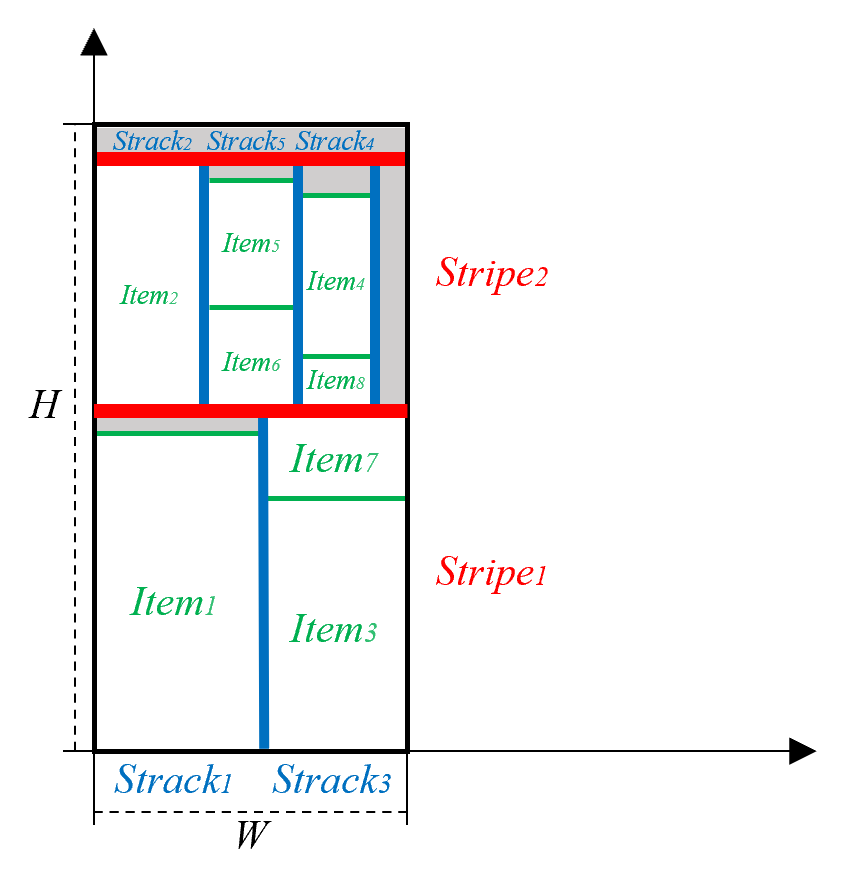
\includegraphics[width=.4\textwidth]{左下角优先排布说明.png}
        \caption{标准排样形式示意图} \label{左下角优先排布说明}
\end{figure}


\textbf{板材及各组成的编号规则} \quad 对于某一可行解决方案,其使用板材数量及排样方案确定,任一板材中所含条带的顺序改变、任一条带中栈的顺序改变、或任一栈中产品项的顺序改变,均不会改变此板材的可利用面积,故不改变整体的板材使用方案及数量。按照$h_1 \geq h_2 \geq ...\geq h_n$的顺序,对产品项进行编号。一个可行解决方案最多包含$n$个栈,取栈所含的最高产品项编号作为此栈的编号,也即所含产品项的最小编号。在此编号规则下,对于栈$j$,可知它一定包含产品项$j$,且产品项$j$为高度最大的项,同时编号小于$j$的产品项均不在此栈中。故这样的编号规则可以给后续建模即计算带来较优的简化,例如变量数的减少。类似的,约定一个解决方案最多有$n$个条带,用条带所含栈中最高栈对应的编号,作为此条带的编号;一个解决方案最多需要$n$个板材,用板材所含条带中最高条带对应的编号,作为此板材的编号。



\subsection{模型建立}

\subsubsection{决策变量}
在4.1节编号规则的约定下,我们定义标志各产品项(Item)、栈(Stack)、条带(Stripe)、板材原片(Bin)之间包含关系的决策变量如下:
\begin{equation}   %\mbox{中文}
    a_{j,i}=
    \begin{cases}
        1, \quad  &  {\rm Item}_i \in   {\rm Stack}_j \\
        0,\quad  &  {\rm Item}_i  \notin   {\rm Stack}_j \\
    \end{cases},\quad j=1,...,n, \quad i=j,...,n  \label{决策变量定义a}
\end{equation}

\begin{equation}
    b_{k,j}=
    \begin{cases}
        1, \quad  &  {\rm Stack}_j \in   {\rm Stripe}_k \\
        0,\quad  &  {\rm Stack}_j  \notin   {\rm Stripe}_k \\
    \end{cases},\quad k=1,...,n, \quad j=1,...,n \label{决策变量定义b}
\end{equation}

\begin{equation}
    r_{l,k}=
    \begin{cases}
        1, \quad  &  {\rm Stripe}_k \in   {\rm Bin}_l \\
        0,\quad  &  {\rm Stripe}_k  \notin   {\rm Bin}_l \\
    \end{cases},\quad l=1,...,n, \quad k=l,...n \label{决策变量定义r}
\end{equation}

在此变量定义下,我们可以计算栈$k$的高度$H(k)$为:
\begin{equation}
    H(k)=\sum_{i=1}^{n} h_i a_{k,i}
\end{equation}


这样引入的模型约束是非线性的,不利于后续的求解。为了获得栈高度的线性表达式,我们引入辅助变量$\delta_{l,i,j}$ ,它表征了产品项$i$对板材$l$中所有条带的高度有影响、并被包含于栈$j$中,其定义如下:
\begin{equation}
    \delta_{l,i,j}=  
    \begin{cases}
        1, \quad  & a_{j,i} r_{l,j}=1\\
        0, \quad  & a_{j,i} r_{l,j}=0
    \end{cases},\quad l=1,...,n-1, \quad i=l+1,...,n
\end{equation}
即,$\delta_{l,i,j} = 1$当且仅当项目i包含在栈$j$中,同时栈$j$包含在条带$j$中(则栈i的高度会影响条带$j$的高度),同时条带$j$在板材$l$中。

则我们可以用线性的方式计算板材$l$的已使用高度:
\begin{equation}
\sum_{i=l}^{n} h_i r_{l,i}+\sum_{i=l+1}^{n} h_i \sum_{j=l}^{i-1} \delta_{l,i,j}
\end{equation}

\subsubsection{方向说明}
为了便于后续讨论,本文规定第一阶段切割方向为x方向,即切割方向垂直于高度、平行于长度的方向,如图\ref{方向说明1},与之垂直的板材原片的边的长度规定为板材原片的高度$H$,平行的边的长度规定为板材原片的长度$W$。
\begin{figure}[!htbp]
    \centering
    \begin{minipage}{0.48\linewidth}
        \centering
        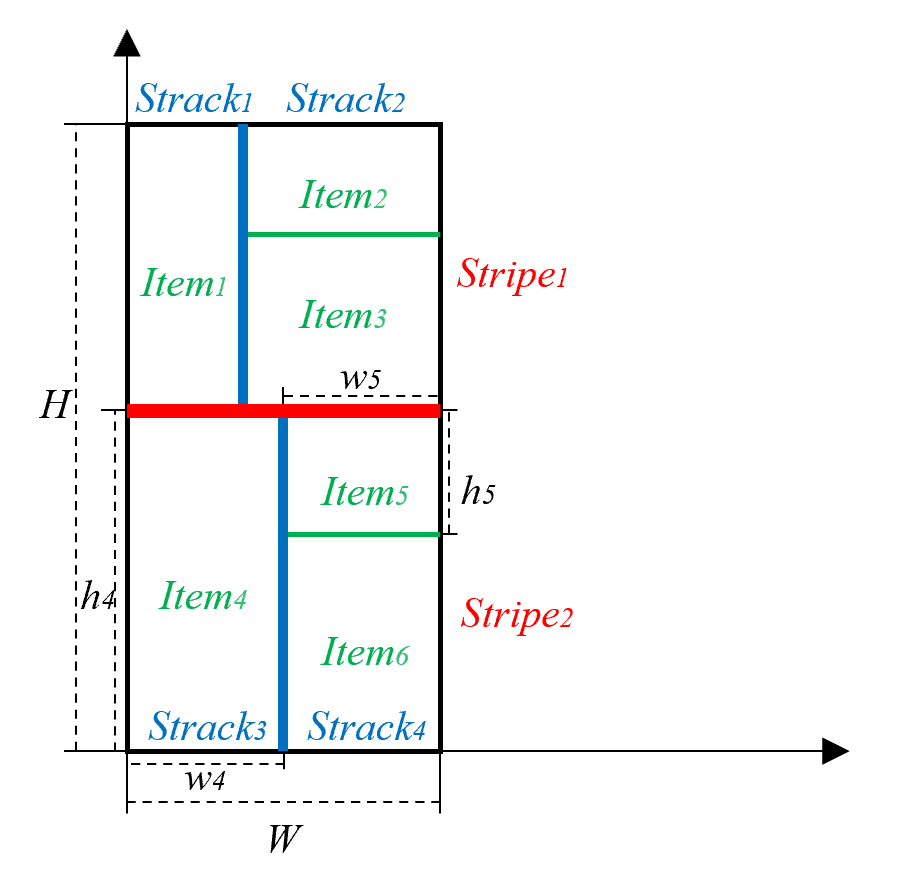
\includegraphics[width=.9\textwidth]{方向说明1.png}
    \end{minipage}
    \begin{minipage}{0.48\linewidth}
        \centering
        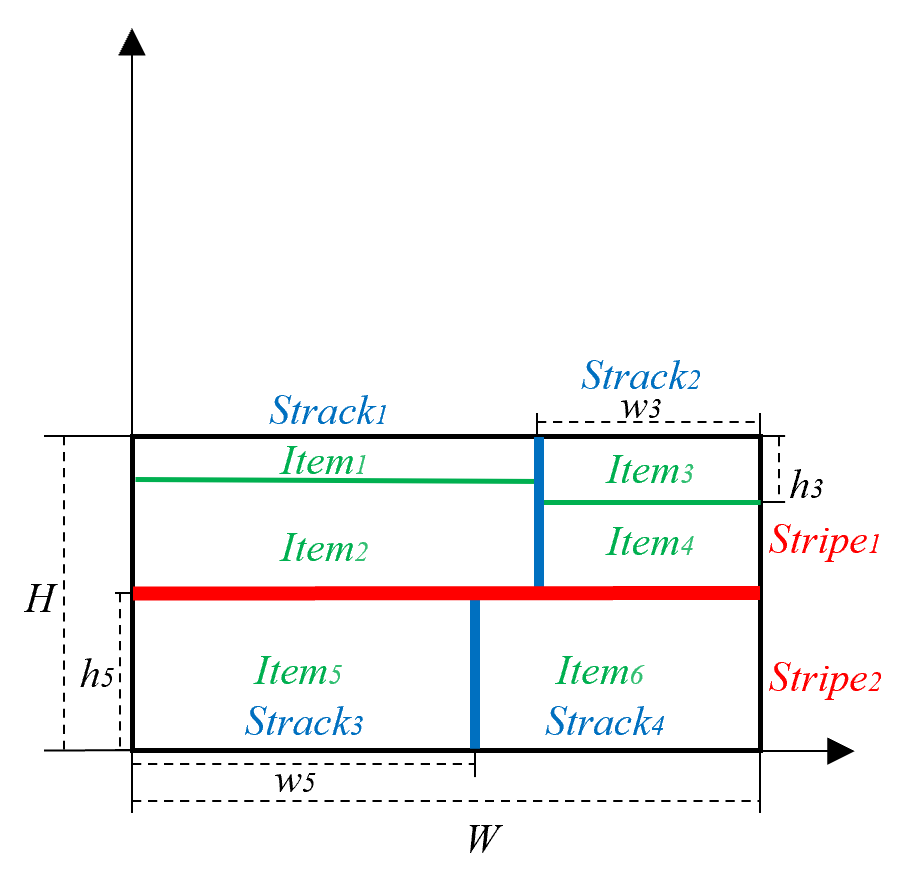
\includegraphics[width=.9\textwidth]{方向说明2.png}     
    \end{minipage}
    \caption{原始板材切割示意图}\label{方向说明1}
\end{figure}


\subsubsection{模型建立}
%根据每次切割均必须垂直于板材边界,易知对于统一板材而言切割只有垂直于高或者垂直于宽两种方向,且各个阶段的切割方向交替进行,即第一阶段与第三阶段切割方向一致,第二阶段切割方向垂直于第一和第三阶段。为便于后续讨论,我们不妨规定在第一阶段完成尽可能多的切割。



优化目标是最小化所使用的板材数量,如4.1节中的问题分析,此目标与题意中的尽可能减少板材用量等价,且更为简洁直观、便于计算。当$ r_{l,l}=1 $时表示板材$l$被使用,则目标函数可如下表示:
\begin{equation}
    min \sum_{l=1}^{n}  r_{l,l} \label{目标函数}
 \end{equation}


根据前述分析,该优化问题涉及变量存在相应约束条件,每个产品项$i$在且仅在一块板材中出现:

\begin{equation}
    \sum_{j=1}^{i}  a_{j,i} =1,\quad \forall i=1,...,n \label{产品项必须排}
\end{equation}


产品项只会被分配给已使用的栈:

\begin{equation}
   \sum_{i=j}^{n}  a_{j,i} \le (n-j+1)a_{j,j},\quad \forall j=1,...,n  \label{产品项只给已使用栈}
\end{equation}

排样在同一栈中的产品项必须具有相同的宽度,并且任何一个栈中的产品项的总高度不得超过板材高度$H$:
\begin{equation}
     a_{j,i}=0, \quad \forall j=1,...,n-1,\quad  \forall i>j \mid w_i \neq w_j \vee h_i+h_j>H \label{相同宽度}
 \end{equation}

已使用的栈$j$在且仅在一条条带$j$中:
\begin{equation}
    \sum_{k=1}^{n}  b_{k,j} =a_{j,j},\quad \forall j=1,...,n  \label{栈精确排在条带}
\end{equation}

每个栈 $j$的高度不超过所在条带 $k$ 的高度,考虑栈高度可能相同的情况,按照“严格小于”和“小于等于”两张情况予以区分:
\begin{equation}
    \sum_{i=j}^{n} h_ia_{j,i}<\sum_{i=k}^n h_i a_{k,i}+(H+1)(1-b_{k,j}),\quad  \forall  k=2,...,n,\quad  \forall j=1,...,k-1 \label{严格小于的高度限制}
\end{equation}
\begin{equation}
    \sum_{i=j}^{n} h_ia_{j,i} \le \sum_{i=k}^n h_i a_{k,i}+H(1-b_{k,j}), \quad  \forall k=1,...,n-1, \quad \forall j=k+1,...,n \label{小于等于的高度限制}
\end{equation}

条带的宽度不超过箱子的宽度,且栈只会被分配给已使用的条带中:
\begin{equation}
    \sum_{j=1}^{n} w_j b_{k,j} \le W b_{k,k}, \quad k=1,...,n \label{宽度限制}
\end{equation}

每个已使用的条带在且仅在一块板材中:
\begin{equation}
    \sum_{l=1}^{k} r_{l,k} = b_{k,k}, \quad \forall k=1,...,n \label{条带精准打包}
\end{equation}

一块板材上条带的总高度不超过板材的高度:
\begin{equation}
    \sum_{i=l}^{n} h_i r_{l,i} +\sum_{i=l+1}^{n} h_i \sum_{j=l}^{i-1} \delta_{l,i,j} \le H r_{l,l}, \quad \forall l=1,...,n-1 \label{板材高度}
\end{equation}

根据决策变量的定义(\ref{决策变量定义a})、定义(\ref{决策变量定义r}),设置辅助变量的值:
\begin{equation}
    a_{j,i}+r_{l,j}-1 \le \delta_{l,i,j} \le (a_{j,i}+r_{l,j})/2, \quad \forall l=1,...,n-1,\quad \forall i=l+1,...,n,\quad j=l,...,i-1 \label{决策变量相关}
\end{equation}

条带只会分配给已使用的板材:
\begin{equation}
    \sum_{k=l+1}^{n} r_{l.k} \le (n-l)r_{l,l}, \quad \forall l=1,...,n-1 \label{未使用板材无条带}
\end{equation}

公式(\ref{范围a})-(\ref{范围delta})为变量的范围,所有变量均为0-1整数型变量:
\begin{equation}
    a_{j,i} \in \{0,1\}, \quad j=1,...,n , \quad i=j,...,n \label{范围a}
\end{equation}
\begin{equation}
    b_{k,j} \in \{0,1\}, \quad k=1,...,n , \quad j=1,...,n \label{范围b}
\end{equation}
\begin{equation}
    r_{l,k} \in \{0,1\}, \quad l=1,...,n , \quad k=l,...,n \label{范围r}
\end{equation}
\begin{equation}
    \delta_{l,i,j} \in \{0,1\}, \quad j=1,...,n-1 , \quad i=l+1,...,n \label{范围delta}
\end{equation}

完整的问题一的\textbf{三阶段2BP二进制整数线性规划模型}如下所示:
\begin{equation}
    \begin{cases}
        min \sum_{l=1}^{n}  r_{l,l} \\
        s.t.
        \begin{cases}
            \sum_{j=1}^{i}  a_{j,i} =1,\quad \forall i=1,...,n \\
            \sum_{i=j}^{n}  a_{j,i} \le (n-j+1)a_{j,j},\quad \forall j=1,...,n  \\
            a_{j,i}=0, \quad \forall j=1,...,n-1,\quad  \forall i>j \mid w_i \neq w_j \vee h_i+h_j>H\\
            \sum_{k=1}^{n}  b_{k,j} =a_{j,j},\quad \forall j=1,...,n  \\
            \sum_{i=j}^{n} h_ia_{j,i}<\sum_{i=k}^n h_i a_{k,i}+(H+1)(1-b_{k,j}),\quad  \forall  k=2,...,n,\quad  \forall j=1,...,k-1 \\
            \sum_{i=j}^{n} h_ia_{j,i} \le \sum_{i=k}^n h_i a_{k,i}+H(1-b_{k,j}), \quad  \forall k=1,...,n-1, \quad \forall j=k+1,...,n \\
            \sum_{j=1}^{n} w_j b_{k,j} \le W b_{k,k}, \quad k=1,...,n \\
            \sum_{l=1}^{k} r_{l,k} = b_{k,k}, \quad \forall k=1,...,n \\
            \sum_{i=l}^{n} h_i r_{l,i} +\sum_{i=l+1}^{n} h_i \sum_{j=l}^{i-1} \delta_{l,i,j} \le H r_{l,l}, \quad \forall l=1,...,n-1 \\
            a_{j,i}+r_{l,j}-1 \le \delta_{l,i,j} \le (a_{j,i}+r_{l,j})/2, \quad \forall l=1,...,n-1,\quad \forall i=l+1,...,n,\quad j=l,...,i-1 \\
           \sum_{k=l+1}^{n} r_{l.k} \le (n-l)r_{l,l}, \quad \forall l=1,...,n-1 \\
            a_{j,i} \in {0,1}, \quad j=1,...,n , \quad i=j,...,n \\
            b_{k,j} \in {0,1}, \quad k=1,...,n , \quad j=1,...,n \\
            r_{l,k} \in {0,1}, \quad l=1,...,n , \quad k=l,...,n \\
            \delta_{l,i,j} \in {0,1}, \quad j=1,...,n-1 , \quad i=l+1,...,n 
        \end{cases}  \label{问题一模型}
    \end{cases}
\end{equation}



%\subsubsection{编号规则}
%
%(1)\textbf{产品项}:将各个产品项按长度从大到小排序后,从1到n依次编号;
%
%(2)\textbf{栈}:用栈中包含产品项的最小编号为该栈编号,若1到n中还有剩余编号,则这些编号分别对应一个不包含任何产品项、也不包含于任何条带的空栈;
%
%(3) \textbf{条带}:用条带中包含栈的最小编号为该条带编号,若1到n中还有剩余编号,则这些编号分别对应一个不包含任何栈、也不包含于任何板材原片的空条带;
%
%(4)\textbf{板材原片}:用板材原片中包含条带的最小编号为该板材原片编号,若1到n中还有剩余编号,则这些编号分别对应一个不包含任何条带(未使用)的空板材原片。
%
%根据上述编号规则,可知
%% (这里注意要不要写成约束)
%
%\begin{equation}
%    h_{1} \ge h_{2} \ge ... \ge h_{n}
%\end{equation} 
%\begin{equation}
%    a_{j,i}=0, \quad   j>i
%\end{equation}
%\begin{equation}
%    b_{k,j}=0, \quad   k>j
%\end{equation}
%\begin{equation}
%    r_{l,k}=0, \quad   l>k
%\end{equation}
%\begin{equation}
%    a_{j,j}=
%    \begin{cases}
%        1, \quad  &  {\rm Stack}_j \neq  \phi  \\
%        0,\quad  &  {\rm Stack}_j  =  \phi  \\
%    \end{cases}
%\end{equation}
%\begin{equation}
%    b_{k,k}=
%    \begin{cases}
%        1, \quad  &  {\rm Stripe}_k \neq  \phi  \\
%        0,\quad  &  {\rm Stripe}_k =  \phi  \\
%    \end{cases}
%\end{equation}
%\begin{equation}
%    r_{l,l}=
%    \begin{cases}
%        1, \quad  &  {\rm  {\rm Bin}}_l \neq  \phi  \\
%        0,\quad  &  {\rm  {\rm Bin}}_l = \phi  \\
%    \end{cases}
%\end{equation}
%
%\subsubsection{目标函数}
%最小化板材原片使用数量:
%\begin{equation}
%    Min \sum_{l=1}^{n} r_{l,l} 
%\end{equation}
%
%\subsubsection{约束条件}
%每个产品项当且仅当出现在一个栈中
%\begin{equation}
%    \sum_{j=1}^{n} a_{j,i}=\sum_{j=1}^{i} a_{j,i}=1
%\end{equation}  
%
%而每个非空栈当且仅当出现在一个条带中
%\begin{equation}
%    \sum_{k=1}^{n} b_{k,j}=\sum_{k=1}^{j} b_{k,j}=a_{j,j}
%\end{equation}  
%
%同理
%
%\begin{equation}
%    \sum_{l=1}^{n} r_{l,k}=\sum_{l=1}^{k} r_{l,k} =b_{k,k}
%\end{equation}  
%
%\begin{equation}
%    \sum_{i=1}^{n} r_{j,i}=1
%\end{equation}  
%
%
%\begin{equation}
%    a_{j,i}=0, \quad   h_{i}+h_{j}>H
%\end{equation}
%\begin{equation}
%    a_{j,i}=0, \quad  w_{i} \ne w_{j}
%\end{equation}
%
%
%\begin{equation}
%    a_{j,j}=1
%\end{equation}
%
%
%\begin{equation}
%    b_{k,k}=1
%\end{equation}
%
%\begin{equation}
%    r_{l,l}=1
%\end{equation}
%
%
%相同栈里的产品项宽度或长度相同
%\begin{equation}
%    \sum_{l=1}^{k} a_{l,k}=1,\quad \forall k\leqslant n
%\end{equation}  
%
%
%通过前述问题分析,我们建立了如下数学模型:
%
%\begin{equation}
%    \begin{aligned}
%    Min \sum_{l=1}^{n} r_{l,l}\\
%    Min \sum_{l=1}^{n} r_{l,l}
%    \end{aligned}
%\end{equation}  
%
%
%\begin{equation}
%    \begin{aligned}
%    Min \sum_{l=1}^{n} r_{l,l}\\
%    Min \sum_{l=1}^{n} r_{l,l}
%    \end{aligned}
%\end{equation}  



\subsection{模型求解}
	
\subsubsection{数学模型特点分析}
	\textbf{数学模型特点} 
	
	1. 变量多、呈 $ n^2 $ 量级 \quad 所建立的二进制整数线性规划模型,如式子(\ref{范围a})-(\ref{范围delta})所示,其变量个数在 $ n^2 $ 数量级,约束为$ n $的多项式数量级,故随着变量数量增加,求解规模将指数级增长,求解时间长甚至难以在有限步内得到解。 题目所给的数据集基本在 $ 10^3 $ 量级,由此对应的模型规模较大。
	
	2. 0-1变量、线性约束 \quad	线性规划求解发展较为成熟,但本模型的变量为0-1二进制整数类型,传统的连续线性规划等方法难以适用。
	
	\textbf{求解方向} \quad 正如4.1节的分析,问题一属于2BP问题,这是一个典型的NP-Hard问题,最优解无法在多项式时间内计算得到。NP-Hard问题有两个求解方向:一是利用传统算法例如分枝定界法、动态规划法等,在指数时间内求最优解;二是利用近似算法、近似方案或启发式算法,例如贪心算法、线性规划松弛、局部搜索、粒子群算法等,在多项式时间内求得近似解。
	
	\textbf{求解算法} \quad 结合NP-Hard可行的求解方向与本模型的特点,决定采用FFFD(Finite First Fit Decrease,有限降序首次适应)算法进行求解。具体思路详见4.3.2节。


\subsubsection{FFFD有限降序首次适应算法}
	\textbf{(1)算法思路}
	
	采用高度降序的顺序将产品项放入有序表中,只要产品项有序表不为空,算法会一个一个将产品项排进板材中。产品项的栈会尽可能长的添加到当前条带中,若当前条带无法再放进任何产品项,则会在当前板材中新增一个空条带,如果没有产品项能放入此新的空条带,则丢弃此空条带,将此板材添加进解决方案,并初始化新板材。
	
	FFFD算法的具体执行逻辑为:
	
	1. 对所有 {\rm Item},按照高度降序排序,放入待排样产品有序表里;
	
	2. 当有序表非空时,创建一个新的板材B,否则跳至6结束程序;
	
	3. 创建一个新的条带记为S,初始化其宽为$W$,高为0,所含栈为空。遍历有序表记当前项为I:
	
	1) 如果S为空,且I可以放进其中,则放入,并将I从有序表中移去、更新S信息;
	
	2) 如果S非空,且I可以放进其中,则放入,并将当前I从有序表中移去、更新条带,然后遍历有序表中的剩余项记为$\rm{I}_2$,若$\rm{I}_2$放入I所在栈的,则将$\rm{I}_2$放入此栈,并将$\rm{I}_2$从List中移去、更新S信息(其中,当条带为空时,产品项能放进此条带的判据是:产品项的宽度小于条带的未使用宽度,且高度小于板材的未使用高度。当条带不为空时,产品项能排进此条带的判据是:当前产品项的宽度小于条带的未使用宽度,且高度小于条带的未使用高度。产品项2能放入某一产品项所在栈的判据是:两个产品项的宽度相同,且产品项2的高度小于此栈所在条带的未使用高度);
	
	4. 如果S不为空,则重复第3步、第4步;
	
	5. 如果S为空,丢弃此空S,将此B添加进可行解方案中,跳至第2步;
	
	6. 结束程序,此时产品项已排完,得到一个可行解方案。
	
	
	\textbf{(2)算法分析}
	
	\textbf{合理性} 
	
	1. 算法流程设计的合理性。排样优化是一个产品项布局最优的静态问题,从动态角度,可将问题转化为:存在某种最优的顺序,当将产品按此顺序逐个放在板材上时,满足切割条件并能实现板材用量最少。FFFD算法从动态视角模拟排样问题最优解的生成过程,理论上若能找到此最优顺序,就可以找到最优解。
	
	2. 降序顺序选取的合理性。从理论上分析,考虑实际排样场景,宽度近似的情况下,高度较长的产品项相比高度较短的产品项,对板材余料的可用性要求更高,即能找到可容纳的板材类型更少。因此优先考虑高度更长的产品项纳入板材排样,由高度小的板材作为灵活插入项,去提高已排长产品项的各板材的使用面积,理论上可一定程度上比随机选取产品项排样效率更好。从实际测试上分析,经多种不同顺序排序的测试,降序排序整体表现最优,故选取此顺序合理。
	
	\textbf{可实现性}  
	
	FFFD算法为有限实现算法,表现为算法在有限步骤内可求得解,因为对产品项有序表遍历,总会实现产品项的放入,无论是直接放入还是新建一个板材再放入。且由算法逻辑可见,程序只有简单的遍历与判断,编写实现难度低。
	
	\textbf{复杂度估计}
	
	该FFFD算法的最好时间复杂度为$O(n)$,最坏时间复杂度为 $ O(n^2) $。
	
	\textbf{运行时间分析}
	 
	由于FFFD为首次可放即放入逻辑,n一般不会增长到较大值即可从有序表中移出,呈现近于O(n)的运行时间量级;且FFFD总是在有限步内求得可行解,故运行时间理论较快。
	
\subsubsection{启发式算法}



\subsection{求解结果}

	运行FFFD算法对数据集A进行求解,800个左右产品项数量的数据集,0.2s左右即可计算完毕,得到结果如表1所示。
    
    \begin{table}[htph]
        \centering
        \caption{问题一 FFFD算法求解结果}
         \label{问题一 FFFD算法求解结果}
        \begin{tabular}{ccccc}
         \hline
         \makebox[0.2\textwidth][c]{数据集}&\makebox[0.16\textwidth][c]{A1}&\makebox[0.16\textwidth][c]{A2}&\makebox[0.16\textwidth][c]{A3}&\makebox[0.16\textwidth][c]{A4}\\ \hline
         产品项总数&752&731&823&799 \\ \hline
         利用率 &0.94933&0.93117& 0.95147&0.94083 \\ \hline
         板材数&88&89&88&87\\ \hline
         FFFD求解耗时(s)&0.18849&0.17247&0.21430 &0.20128 \\ \hline 
        \multicolumn{5}{l}{【注】:板材利用率 = 产品项面积之和 / 使用原片面积之和}\\
        \end{tabular}
        \end{table}
	
	所得利用率均在93\% 以上,表明FFFD算法获得了较为不错的结果。同时可求得各板材的产品项排样方案,见附录。
	
	
\subsection{模型及算法评价}





\section{问题二订单组批}

\subsection{问题分析}
该问题中要求订单当且仅当出现在一个批次中,即订单不可拆分,所以该问题也可简述为在问题一的基础上完成订单的组合问题。这仍然是一个NP-Hard问题,若简单沿用问题一的混合整数线性规划模型(\ref{问题一模型}),引入新的变量与约束,这会使得模型求解难度进一步增大,求解时间增长,显然这并非是解决该问题合适的方法。

因此,本问题将在问题一的基础上,进一步建立\textbf{两步优化模型},内层模型求解最优排样方案,外层模型求解最优组批方案,显然这是一个带有线性约束及非线性目标函数的混合整数非线性规划问题。

\subsection{模型建立}


\subsubsection{决策变量}

类似问题一中(\ref{决策变量定义a})、(\ref{决策变量定义b})、(\ref{决策变量定义r})的变量定义方法,定义批次的编号为该批次所包含的最小的订单编号,则有描述各批次(Batch)、订单(Order)之间包含关系的决策变量如下:
\begin{equation}   %\mbox{中文}
    d_{q,p}=
    \begin{cases}
        1, \quad  & \text{Order}_p \in  \text{Batch}_q \\
        0,\quad  & \text{Order}_p \notin  \text{Batch}_q \\
    \end{cases},\quad q\le p \le m,\quad p,q \in  \mathbb{N}^+\\
\end{equation}
\noindent 式中,$m$为订单总数。


\subsubsection{模型建立}
该问题目标函数为总的板材利用率最高,为总原始板材使用数量最少。

\textbf{定义}非线性函数$f_q(d_{q,1},d_{q,2},\cdots,d_{q,m})$,表示在第$q$批次的订单组合$(d_{q,1},d_{q,2},\cdots,d_{q,m})$利用问题一模型所求得的最佳排样方案所使用的原始板材数量。

即有非线性目标函数
\begin{equation}   
    \mathbf{min}\quad\sum_{q=1}^{m} f_q(d_{q,1},d_{q,2},\cdots,d_{q,m}),q\le m ,q\in  \mathbb{N}^+\label{目标函数2}
\end{equation}

该目标函数中,函数$f_q$可利用问题一模型求解,函数$f_q$的优化求解问题,即为该组批优化的内层优化问题。

等式约束(\ref{订单必须排})保证所有的订单$p$被批次$q$包含且仅包含1次。

\begin{equation}   
    \sum_{q=1}^{p} d_{q,p}=1,\quad \forall p\le m,p \in \mathbb{N}^+ \label{订单必须排} 
\end{equation}


在$d_{q,p}$的编号原则约定下,不等式约束\ref{编号原则2}保证订单$p$仅分配给非空的批次$q$。

\begin{equation}   
\sum_{p=q}^{m} d_{q,p} \le (m-q+1)d_{q,q},\quad \forall q\le m,q\in \mathbb{N}^+\label{编号原则2}
\end{equation}

\textbf{定义}$n_p$为订单p所包含的产品项个数,为保证加工环节快速流转,每个批次产品项(item)总数不能超过限定值,则有

\begin{equation}   
    \sum_{p=q}^{m} n_pd_{q,p} \le \text{max\_item\_num},\quad \forall q \le m, q\in \mathbb{N}^+
\end{equation}

\textbf{定义}$S_p$为订单p所包含的产品项总面积,因工厂产能限制,每个批次产品项(item)的面积总和不能超过限定值,所以有

\begin{equation}   
    \sum_{p=q}^{m} S_pd_{q,p} le max\_item\_area,\quad \forall q\le m,q\in \mathbb{N}^+
\end{equation}

因此,可以得到混合整数非线性规划模型
\begin{equation}
    \begin{cases}
        \mathbf{min} \sum_{q=1}^{m} f_q(d_{q,1},d_{q,2},\cdots,d_{q,m}) \\
        \mathbf{s.t.}
        \begin{cases}
            \sum_{q=1}^{p} d_{q,p}=1,\quad \forall p\le m,p \in \mathbb{N}^+ \\
            \sum_{p=q}^{m} d_{q,p} \le (m-q+1)d_{q,q},\quad \forall q\le m,q\in \mathbb{N}^+  \\
            \sum_{p=q}^{m} n_pd_{q,p} \le \text{max\_item\_num},\quad \forall q \le m, q\in \mathbb{N}^+\\
            \sum_{p=q}^{m} S_pd_{q,p} le max\_item\_area,\quad \forall q\le m,q\in \mathbb{N}^+ \\
        \end{cases}  \label{问题二模型}
    \end{cases}
\end{equation}


\subsection{模型求解}
\subsubsection{数学模型特点分析}
	\textbf{数学模型特点} 
	
    该数学模型外层模型为混合整数非线性模型,与问题一类似,该数学模型仍然具有变量多、量级重的问题,变量数量呈 $ n^2 $ 量级。此外,由于该模型为两步优化模型,所以内层模型的优化速度也极大程度的影响了整个模型的迭代求解过程。
	
	\textbf{内层模型求解} 由于内层模型的计算速度和准确性极大程度的影响了全局模型的优化效率和效果,所以综合考虑此处内层模型使用问题一4.3.2节中FFFD算法求解。
	
	\textbf{外层模型求解} 传统算法仍难以解决该类大规模混合整数非线性规划问题,设计合适的贪心算法并求得该模型的局部最优解,仍然是求解该模型的关键。

\subsubsection{优先搜索算法设计}
该算法旨在解决订单组批问题,为了后文更好的描述求解算法,将该问题做如下描述:现总共有$m$个生产批次,每个生产批次仅含1个订单,通过合适的方法,将多个批次组合为1个批次,从而降低板材使用数量,提高板材利用率。

在解决该一般问题之前,先考虑一组特异性数据。

\textbf{特异性问题}

1)假定在所有产品项中材质$t$的产品项有且仅有2个,分别被2个批次$\text{Batch}_1$、$\text{Batch}_2$包含,且两个产品项可排样在1块原始板材上。

显然,当且仅当这2个批次被组合到一起时,该材质所使用的原始板材数量才会减少。否则,该材质的板材利用率不会再提高。

2)相反地,对于产品项数量更多的材质$t'$,其被批次$q'$等多个批次所包含。

此时,如若因为约束等因素限制,使得这些批次中两个或几个批次不能再次与批次$q'$组合。但是仍然可能会有其他可选批次与订单$p'$组合,并提高其板材利用率。而且由于其产品项数量多、形状多,在排样时可选方案也更多,该类材质往往能有较高的板材利用率。

因此,在此种情况下,情况1)中的订单组合到同一个批次中带来的收益往往会大于情况2)中的订单组合。换言之,在组合订单时,情况1)中的订单可以优先考虑。

\textbf{一般问题}

基于以上讨论,可以得出经验性结论,即当材质$t$的产品项被尽可能的少的批次所包含、且材质$t$的产品项能够被排样到尽可能的少的原始板材时,包含材质$t$的产品项的批次在组合时应有更高的优先级。

因此,为解决该一般问题,可以将合并后能够产生收益(使得该类材质使用的原始板材数量减少,例如特异性问题中的情况1))且满足题目约束的两个此类批次优先整合到一起。组合后,这两个批次转换为一个批次,于是,该问题再次转变为批次组合问题,可以继续以相同的方式,对剩下的批次进行组合,直到剩下的批次中任意两个组合在一起都不能继续提高板材利用率。



\subsubsection{优先搜索算法步骤}
1)假定在所有订单中材质$t$的产品项有且仅有2个,分别被2组订单$\text{Order}_1$、$\text{Order}_2$包含,且两个产品项可排样在1块原始板材上。

显然,当且仅当这2组订单被组合到同一批次中,该材质所使用的原始板材数量才会减少。如果2组订单被分配到不同的批次中,则该材质的板材利用率不会再提高。

2)相反地,对于数量更多的材质$t'$,其被订单$p'$等大批量组订单所包含。

此时,如若出现与1)中相同的情况,其中两个或几个订单被分配到不同批次。仍然会有其他可选批次与订单$p'$组合,并提高其板材利用率。而且由于其产品项数量多、形状多,在排样时可选方案也更多,该类材质往往能有较高的板材利用率。

接下来讨论一般问题



\subsubsection{优先搜索算法}
1) 初始化订单$p$的生产批次为第$q=p$批。

2) 对每种材质全部产品项进行排样,并按照其所需的排序,排在前位的材质中的批次,合并为一个批次的优先级更高。

3) 按照第2)步形成的材质顺序进行搜索,对于材质t,如果包含材质t的批次不少于2个,则考虑其任意2个批次合并后,是否可以有效的减少该材质t的原始板材使用数量。

4) 如果可以减少该材质t的原始板材使用数量,同时2个批次合并后不违反单个批次产品项综述约束及面积总和约束,则将该2个批次合并,回到步骤2) 重新排样并排序。否则,回到步骤3) 继续搜索下一材质。

5) 当全部材质搜索结束,这说明此时任何两个批次合并到一起,都不会再减少总的板材使用数量,即无法进一步提高板材利用率。此时,得到订单组批方案。

6) 对不连续的批次编号重新整理、编号,输出求解结果。

7) 此时的订单组批方案中,并非所有批次都接近单个批次产品项总数上限或面积总和上限,其小规模的批次仍完成可进一步合并,以减少批次数量。然而,考虑到此种合并不会进一步提高板材利用率,与本文的优化目标无关,且这种组合方法可以较易实现,因此,本文不再考虑对批次的进一步合并的问题。

算法\ref{test}
\begin{algorithm}
    % \SetAlgoNoLine
    \caption{Put your caption here}\label{test}
    \begin{multicols}{2}
        \SetAlgoLined
        \KwData{this text}
        KwResult{how to write algorithm with \LaTeX2e }
        initialization\;
        \While{not at end of this document}{read current\;
        \eIf{understand}
        {go to next section\;current section becomes this one\;
        }{
        go back to the beginning of current section\;
        }
        }
    \end{multicols}
\end{algorithm}

\subsection{求解结果}

	运行算法对数据集B进行求解,所得结果如表\ref{问题二 优化搜索算法求解结果}所示。
    \begin{table}[htph]
        \centering
        \caption{问题二 优化搜索算法求解结果}
         \label{问题二 优化搜索算法求解结果}
        \begin{tabular}{cccccc}
         \hline
         \makebox[0.2\textwidth][c]{数据集}&\makebox[0.12\textwidth][c]{B1}&\makebox[0.12\textwidth][c]{B2}&\makebox[0.12\textwidth][c]{B3}&\makebox[0.12\textwidth][c]{B4}&\makebox[0.12\textwidth][c]{B5}\\ \hline
         利用率&0.79231&0.77665&0.77942& 0.78172&0.76591 \\ \hline
	     批次数&44&35&34&35&45 \\ \hline
         板材总数&3759&2481&2620&2597&4034 \\ \hline
         求解耗时(s)&0&0&0&0&0\\ \hline
         
        \end{tabular}
        \end{table}
    
		

	所得利用率在 76\% \~ 80\% 之间,相比问题一较低,这主要由于同一订单的产品项必须在相同批次,而材质不同的产品项无法排样在同一块板材原件上所导致。由输出结果所得各组批的排样图分析可见,在此组批约束下,此排样结果已相对较优。各组批方案详见附录。

\section{模型评价与展望}





\newpage
\quad
\newpage

%参考文献   手工录入
%\begin{thebibliography}{9}%宽度9
% \bib {\rm Item}{bib:one} ....
% \bib {\rm Item}{bib:two} ....
%\end{thebibliography}

%采用bibtex方案
\bibliographystyle{gmcm}
\bibliography{MCM_2022}

\cite{mittelbach_latex_2004,wright_latex3_2009,beeton_unicode_2008,vieth_experiences_2009}

\newpage
%附录
\appendix
\setcounter{page}{1} %如果需要可以自行重置页码。
\section{数据预处理及读取函数}
\lstinputlisting[language=matlab]{../code/data_pre_fun.m}
\section{问题一主程序}
\lstinputlisting[language=matlab]{../code/q1_main.m}
\section{问题一FFF算法}
\lstinputlisting[language=matlab]{../code/q1_FFF_fun.m}
\section{问题二主程序}
\lstinputlisting[language=matlab]{../code/q2_main.m}
\section{问题二XX算法}
\lstinputlisting[language=matlab]{../code/q2_tanlan.m}
\section{将计算结果保存至文件}
\lstinputlisting[language=matlab]{../code/save_to_file_fun.m}
\section{绘制排样图至文件}
\lstinputlisting[language=matlab]{../code/draw_picture_fun.m}

\end{document} 